\documentclass[smallabstract,smallcaptions]{dccpaper}

\usepackage{amsmath}
\usepackage{amssymb}
\usepackage{amsxtra}
\usepackage{latexsym}
\usepackage{cite}
\usepackage{booktabs}
\usepackage[pdfpagemode=UseNone,pdfstartview=FitH,pdfview=FitH,colorlinks=true,
 pdftitle=Daala,pdfauthor=Xiph.Org]{hyperref}
\usepackage{color}
\usepackage{url}
\usepackage{caption}
\usepackage{subcaption}
\usepackage{graphicx}

%\newif\ifpdf
%\ifx\pdfoutput\undefined
%\pdffalse
%\else
%\pdfoutput=1
%\pdftrue
%\fi
%\ifpdf
%\pdfcompresslevel=9
%\providecommand{\figinput}[1]{\input{#1.pdftex_t}}
%\usepackage[pdftex]{graphicx}
%\DeclareGraphicsRule{.pdftex}{pdf}{.pdftex}{}
%\else
%\providecommand{\figinput}[1]{\input{#1.pstex_t}}
%\usepackage{graphicx}
%\DeclareGraphicsRule{.pstex}{eps}{.pstex}{}
%\fi

\newlength{\figurewidth}
\newlength{\smallfigurewidth}


%%%%%%%%%%%%%%%%%%%%%%%%%%%%%%%%%%%%%%
% One Column
%%%%%%%%%%%%%%%%%%%%%%%%%%%%%%%%%%%%%%
\setlength{\smallfigurewidth}{2.75in}
\setlength{\figurewidth}{6in}

\begin{document}

\title
{\large
\textbf{Daala: A Perceptually-Driven Next Generation Video Codec}
}

\author{%
Author One$^{\ast}$, Jean-Marc Valin$^{\ast\dag}$,
 and Timothy B. Terriberry$^{\ast\dag}$\\[0.5em]
{\small\begin{minipage}{\linewidth}\begin{center}
\begin{tabular}{ccc}
$^{\ast}$Xiph.Org Foundation & \hspace*{0.5in} & $^{\dag}$Mozilla \\
21 College Hill Road && 331 E. Evelyn Ave. \\
Somerville, MA 02144, USA && Mountain View, CA 94041, USA\\
\url{tterribe@xiph.org} && %\url{email@address}
\end{tabular}
\end{center}\end{minipage}}
}

\maketitle
\thispagestyle{empty}


\begin{abstract}
The Daala project is an attempt to design a royalty-free video codec capable of
 competing with the best patent-encumbered codecs.
Part of our strategy is to replace core tools of traditional video codecs with
 alternative approaches, many of them designed to take perceptual aspects into
 account, rather than optimizing for simple metrics like PSNR.
This paper documents some of our experiences with these tools, which ones
 worked and which did not, and what we've learned from them.
The result is a codec which compares favorably with HEVC on still images, and
 is on a path to do so for video as well.
\end{abstract}

\Section{Introduction}

This document follows formatting specified in the \textit{DCC Call for Papers};
top margin 1 inch, left margin 1.25 inches, text area 9 inches high by
6 inches wide, single-column, 12 point type. Submissions in response
to the DCC call may not be more than 10 pages (including all figures,
tables, and appendices).

\Section{Headings}

The \LaTeX class for DCC includes formatting for sections \dots

\SubSection{A Subsection Heading}

and also for subsections. The use of sub-subsections is discouraged.

\Section{Figures and Tables}

The proceedings are published in black and white; all figures and
charts should be clear when printed in grayscale. Figures and tables
should be concise and easy to read. Avoid making complex graphics and
then reducing them so much that they become hard to read.

Position illustrations at the top of the page rather than in the middle
or at the bottom. Caption and number every illustration.
Fig.~\ref{fig:example} shows an example illustration.
Table~\ref{tab:example} shows an example table.


\begin{figure}[t]
\begin{center}
\begin{tabular}{cc}
\multicolumn{2}{c}{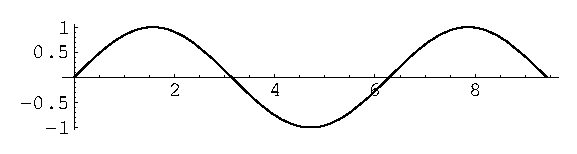
\includegraphics[width=4in]{image1}} \\
\multicolumn{2}{c}{\small{(a)}} \\[1em]
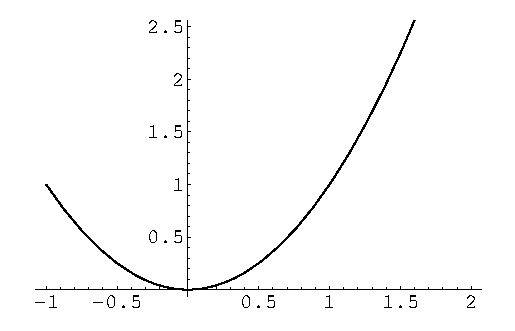
\includegraphics[width=2in]{image3} &
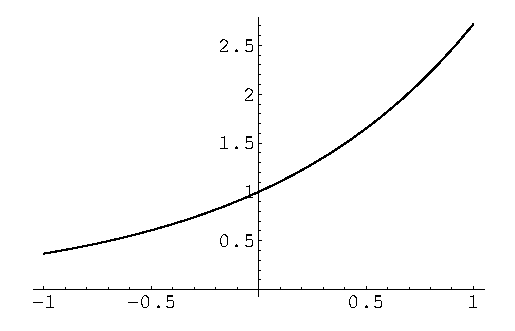
\includegraphics[width=2in]{image4} \\
{\small (b)} & {\small (c)}
\end{tabular}
\end{center}
\caption{\label{fig:example}%
An example figure.}
\end{figure}

\begin{table}[tp]
\begin{center}
\caption{\label{tab:example}%
Average PSNR in dB for the ``Coastguard'' video sequence}
{
\renewcommand{\baselinestretch}{1}\footnotesize
\begin{tabular}{|c|c|c|c|c|}
\cline{2-5}
\multicolumn{1}{c|}{~}&
\multicolumn{1}{c|}{2D} &
\multicolumn{1}{c|}{3D} &
\multicolumn{2}{c|}{MC-BCS-SPL}\\
\cline{4-5}
\multicolumn{1}{c|}{$S_{\text{NK}}$} &
BCS-SPL & BCS-SPL & $S_{\text{K}}=S_{\text{NK}}$ & $S_{\text{K}}=0.7$\\
\hline
0.1 &22.69 &22.76 &23.06 &25.29 \\
0.2 &24.70 &24.76 &25.78 &27.94 \\
0.3 &26.37 &26.45 &28.29 &30.15 \\
0.4 &27.99 &27.95 &30.88 &32.30 \\
0.5 &29.60 &29.57 &33.58 &34.42 \\
\hline
\end{tabular}}
\end{center}
\end{table}

\Section{Reference to Prior Literature}

List and number all bibliographical references at the end of the
paper. The references can be numbered in alphabetic order or in
order of appearance in the document. When referring to them in
the text, type the corresponding reference number in square
brackets as shown at the end of this sentence \cite{Fow2009}.
The reference list below shows an example of citing a
journal article \cite{Fow2009}, a conference paper \cite{Fow2008},
a book chapter \cite{FD2011}, and a book \cite{Par1998}.
Add your citations to the \url{refs.bib} file.

\Section{References}
\bibliographystyle{IEEEtran}
\bibliography{daala-dcc16}

\end{document}
